 
 
 \begin{figure}  
 	\centering
 	\subfigure[System Preference]{
 		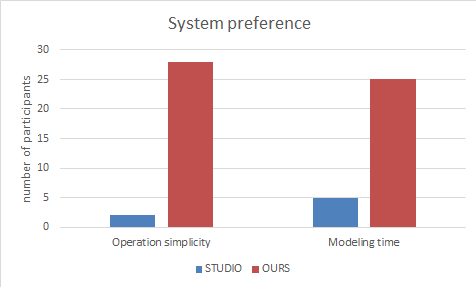
\includegraphics[width=0.25\columnwidth,height=0.11\textheight]{images/preference.png}
 		\label{fig:preference}
 	}
 	\vspace{2ex}
 	\subfigure[Layout Refinment]{
 		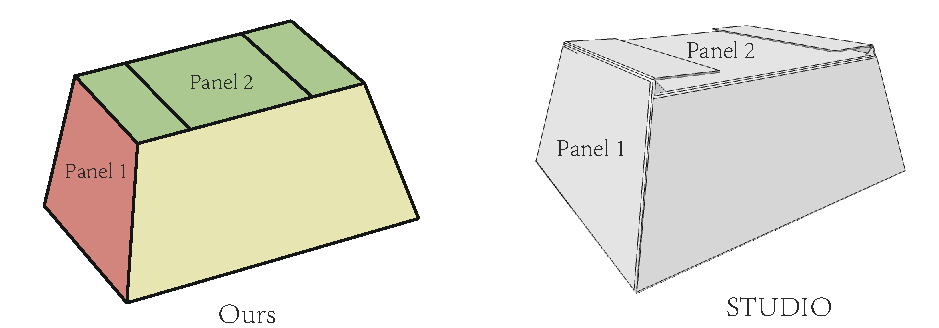
\includegraphics[width=0.35\columnwidth,height=0.08\textheight]{images/comparison}
 		\label{fig:correction}
 	}
 	\vspace{2ex}
 	\subfigure[Fabrication Time]{
 		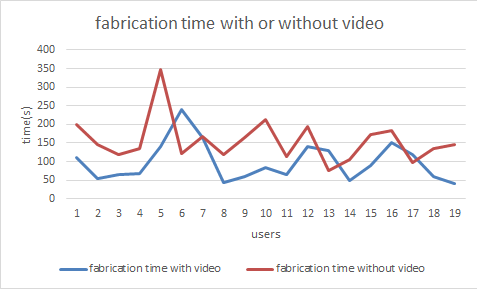
\includegraphics[width=0.25\columnwidth,height=0.11\textheight]{images/fabrication.png}
 		\label{fig:time}
 	}
 	\caption{(a) Compared with STUDIO, more participants prefer our system with regard to both the operation simplicity and modeling time. (b) Our system is able to automatically refine the inaccurate 2D layout, while STUDIO only generates the folded shape based on user assigned angles. (c) Comparison of fabrication times with/without video. It took much longer for common users to fabricate a carton from a 2D layout without our guide.}
 	\label{fig:userstudy}
 \end{figure}
 
 
 
We conducted a user study to examine the productivity of our system for constructing digital 3D mockups from 2D layouts and to analyze the effectiveness of our system in guiding non-expert users to fabricate physical mockups from 2D layouts. 
%
There are two experiments in our user study.
% 
In the first experiment, participants were given a brief introduction, and then they were asked to construct a digital 3D model from the same 2D layout using our system and the commercial software, STUDIO, respectively.
For each participant, 10 examples were randomly selected from the 34 2D design layouts and presented to the participant for folding using our system and Studio.
A \emph{two-alternative forced choices} design was used, so the participant was asked to choose which of the two systems they would prefer to use considering operation simplicity and modeling efficiency. 
%
Furthermore, participants were asked to rate the necessity of layout optimization in our system by using a scale from one to five, with five indicating that it is very necessary.

%
In the second experiment, participants were separated equally into two groups. One group was asked to fold a sheet of paper into a physical carton. The 2D layout was printed onto this piece of paper, and the user was guided by a video showing the folding sequence according to our system. Another group was asked to make a carton without the guide video. 
Each participant was assigned with the same 2D layout (Figure~\ref{fig:automatic-more}(a)), because it is not easy to imagine the final mockup from the 2D layout at first sight.
%
The fabrication times were recorded for the two groups.
%

Based on the two experiments, our goal was to test the following hypotheses:

\begin{itemize}
	\item \textbf{Hypo1:} Our system takes less time and effort to construct a digital 3D mockup than the traditional software.
	\item \textbf{Hypo2:} Our system provides novel and practical functions for generating diverse layouts.
	\item \textbf{Hypo3:} Our system is effective for guiding non-expert users to fabricate complex cartons from 2D layouts.
\end{itemize}




We consider our three hypotheses in turn. 
With respect to \textbf{Hypo1}, we collect the answers to the former two questions from 30 participants, all over eighteen years of age. Both male and female participants were included, and none had any prior experience with designing or folding cartons in computer software. 
%
The results are shown in Figure~\ref{fig:preference}. 
The chart shows that $93\%$ of participants prefer our system with regard to the operation simplicity, and $83\%$ of participants prefer our system with regard to the modeling time.
%
We also performed a paired-samples $t$-test at the level $\alpha = 0.05$ to compare the preference significance.
%
This test shows that our system is significantly preferred by participants.
%
Most participants voted for our system because it takes much less time to make a 3D model using our system. 
Take Figure~\ref{fig:result-more}(e) for example, participants usually spent much time adjusting the folding angles of the creases, while only three clicks are required in our system.
%
On the other hand, one comment from the participants who preferred STUDIO stated that the operation in STUDIO only required them to select and assign angles, while our system required them to learn more operations to construct the digital 3D model. 
%

With respect to \textbf{Hypo2}, 24 participants gave the highest score to our layout optimization function. 
%
In addition to exploring the diversity of 2D layouts, our system can also adjust the imprecise panels on the 2D layout to reach an ideal model. Figure~\ref{fig:correction} shows the final models constructed by our system and STUDIO, respectively. As we can see, Panel 1 is higher than Panel 2 in the digital model constructed by STUDIO, because the 2D layout is not as precise as the designer would like. 
%
In comparison, our system is able to correct these design errors by merging the 3D vertexes in different panels, which are circled in red. This step optimizes the corresponding 2D layout.
 
 
Considering \textbf{Hypo3}, 38 participants (19 in each group) were asked to transform the 2D layout shown in Figure~\ref{fig:automatic-more}(a) into a physical carton. 
The comparison of the fabrication times with and without our guide video is shown in Figure~\ref{fig:time}. 
As we can see, most participants who did not watch the guide video spent more time, averaging 155 seconds, to fold a carton than the other group, averaging 99 seconds.
% 
%
We also performed an independent-samples $t$-test at the level $\alpha = 0.05$ to compare the fabrication times. The results show that the guide video is a highly effective tool for non-expert users in fabricating complex cartons. 


